Das Logical Link Control and Adaption Protocol (L2CAP) bildet die unterste Schicht im Host (siehe S. \pageref{fig: host controller architektur} Abb. \ref{fig: host controller architektur}) und dient je nach Konfiguration dazu, den Datenverkehr zu steuern und zwischen höheren und niedrigeren Schichten zu vermitteln. Mittels Multiplexing können mehrere Anwendungen einen LE-U (also Logical Link) nutzen.
% TODOOPT QUELLE Spec 4.0 S. 1400 2.3 Operation Between Layers
Es verfügt über fünf Modi:
\begin{itemize}
    \item Basic L2CAP Mode
    \item Flow Control Mode
    \item Retransmission Mode
    \item Enhanced Retransmission Mode
    \item Streaming Mode
    \item LE Credit Based Flow Control Mode (seit Bluetooth 4.2)
\end{itemize}
Für Bluetooth allgemein (BR/EDR und LE) wird immer der Basic L2CAP Mode genutzt, wenn kein anderer festgelegt wird. Der LE Credit Based Flow Control Mode soll \cite{BtSpec4.2_1735} zufolge als einziger Modus für verbindungsorientierte LE-Kanäle genutzt werden ("`This is the only mode that shall be used for LE L2CAP connection oriented channels"' \cite{BtSpec4.2_1735}). Da diese Aussage nicht ausschließt, dass eine verbindungsorientierte LE-Verbindung über den standardmäßig festgelegten Basic L2CAP Mode erfolgen kann, und der LE Credit Based Flow Control Mode noch nicht in der Bluetooth-Version 4.0 vertreten war \cite{BtSpec4.0_1401}, ist anzunehmen, dass eine verbindungsorientierte LE-Verbindung auch mit dem Basic L2CAP Mode möglich ist.
% QUELLE ZITAT Spec. 4.2 S. 1735
% QUELLE Spec 4.0 S. 1401
\\\\
Logische Kanäle, genannt L2CAP Channels, dienen innerhalb eines Geräts als Endpunkt für höher gelegene Protokolle oder direkt für die Anwendung und sind für jedes Gerät individuell an dem Channel Identifier (CID) unterscheidbar. Folglich muss der L2CAP Channel einer Verbindung zwischen zwei Geräten von diesen nicht zwingend mit der gleichen CID gekennzeichnet sein.
% TODOOPT QUELLE Spec. 4.0 S. 1390
\\\\
Der L2CAP Layer wird von zwei Modulen gesteuert: dem Resource Manager und dem Channel Manager (siehe Abb. \ref{fig: l2cap architektur}).

\begin{figure}[H]
    \centering
    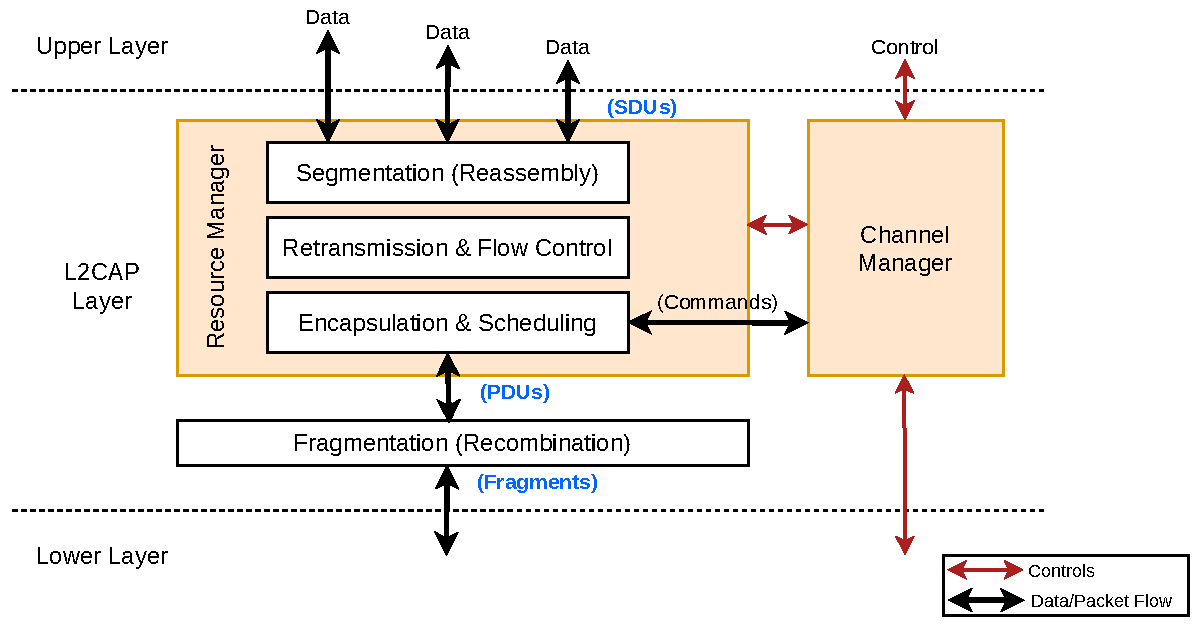
\includegraphics[width=0.9\textwidth]{graphics/l2cap_architektur.pdf}
    \caption[Architektur des L2CAP Layer]{Architektur des L2CAP Layer \cite{BtSpec4.0_1391}}
    \label{fig: l2cap architektur}
\end{figure}
% QUELLE l2cap layer resource manager channel manager spec 4.0 S. 1391

Der Channel Manager ist für die Verwaltung und Steuerung der L2CAP Channels zuständig. Das umfasst die auf L2CAP bezogene Signalübertragung intern, Peer-to-Peer, und zu höheren und niedrigeren Schichten \cite{BtSpec4.0_1390}. 
% QUELLE Spec. 4.0 S. 1390
Die Signale, die zwischen den zwei L2CAP-Entitäten zweier verbundenen Geräte übertragen werden, sind Kommandos wie bspw. der LE Credit Based Connection Request und die entsprechende Response. Dafür wird ein separater L2CAP Channel mit der CID 0x0005 genutzt. Zudem betreibt der Channel Manager den L2CAP-Zustandsautomaten, auf den hier nicht näher eingegangen werden soll.
\\\\
Da der L2CAP Layer nach unten mit dem Link Layer verknüpft ist (ggf. über das HCI), müssen die L2CAP PDUs dem Paketformat des Link Layers (bzw. dem HCI) gerecht werden. Dementsprechend werden die L2CAP PDUs fragmentiert bzw. wieder zusammengesetzt. Die Maximal PDU Payload Size (MPS) bezeichnet die maximale Größe des Payload einer PDU in Byte, die eine L2CAP-Entität verarbeiten kann.
% TODOOPT BILD + VERWEIS Spec 4.0 S. 1487, Mischung aus Figure 7.1 und 7.2, vereinfacht darstellen: L2CAP PDU -> HCI Paket -> Link Layer Paket
\\\\
Ein Datenaustausch zwischen L2CAP und dessen höhergelegenen Schichten / Protokollen erfolgt in der Form von Service Data Units (SDU), wobei deren Ursprung immer aus einer höheren Schicht stammt. Die Maximum Transmission Unit (MTU) bezeichnet die maximale Größe einer SDU in Byte, die die höhergelegene Schicht verarbeiten kann. Die Segmentierung (bzw. Zusammensetzung) dieser SDUs wird vom Resource Manager ausgeführt und ist für alle Modi außer dem Basic L2CAP Mode relevant. Wenn keine Segementierung angewandt wird, ist die MTU gleich der MPS \cite{BtSpec4.2_1727}. Falls ein L2CAP Channel in einem anderen Modus als dem Basic L2CAP Modus agiert, ist der Resource Manager auch für die erneute Übertragung von PDUs und Flusskontrolle zuständig. Außerdem plant der Resource Manager zu welchem Zeitpunkt L2CAP Channel PDUs versenden können, um den L2CAP Channels mit Quality-of-Service-Optionen genügend Ressourcen bezüglich der Buffer des Controllers freizugeben. \cite{BtSpec4.2_185} \cite{BtSpec4.2_1725-1726}

\paragraph{Struktur eines Datenpakets} \mbox{} \vspace{0.2cm} \\
Es existieren verschiedene Arten von L2CAP-Datenpaketen, die den gennanten Modi zugeordnet sind. Der Basic L2CAP Mode unterstützt verbindungsorientierte und verbindungslose L2CAP Channel, während die restlichen Modi nur verbindungsorientierte L2CAP Channels nutzen.
In Abb. \ref{fig: l2cap pdu basic} ist die Paketstruktur einer L2CAP PDU im Basic L2CAP Mode (verbindungsorientiert) dargestellt.

\begin{figure}[H]
    \centering
    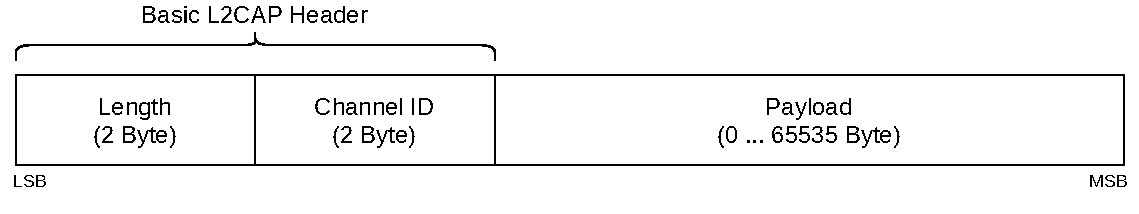
\includegraphics[width=0.9\textwidth]{graphics/l2cap_datenpaket.pdf}
    \caption[Struktur einer L2CAP PDU (Basic L2CAP Mode)]{Struktur einer L2CAP PDU (Basic L2CAP Mode) \cite{BtSpec4.2_fig_1737}}
    \label{fig: l2cap pdu basic}
\end{figure}
% QUELLE Spec. 4.2 S. 1737 Figure 3.1

LSB steht für Least Significant Bit, also das Bit mit niedrigstem Stellenwert, und MSB für Most Significant Bit, also das Bit mit höchstem Stellenwert. Das Längenfeld beschreibt die Länge des Payload, der eine maximale Länge von 65535 Byte besitzt.
\\\\
Abb. \ref{fig: l2cap pdu credit} zeigt die Paketstruktur einer L2CAP PDU im LE Credit Based Flow Control Mode.

\begin{figure}
    \centering
    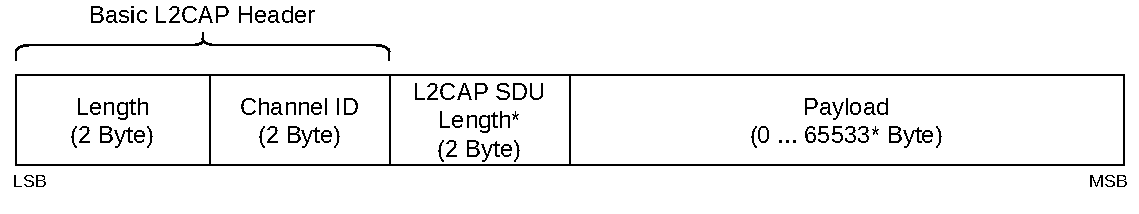
\includegraphics[width=0.9\textwidth]{graphics/l2cap_datenpaket_credit_based.pdf}
    \caption[Struktur einer L2CAP PDU (LE Credit Base Flow Control Mode)]{Struktur einer L2CAP PDU (LE Credit Base Flow Control Mode); *nur in erster PDU einer SDU; \cite{BtSpec4.2_fig_1747}}
    \label{fig: l2cap pdu credit}
\end{figure}
% QUELLE Spec 4.2 S. 1747 Figure 3.6

Das SDU-Längenfeld ist nur in der ersten PDU einer SDU enthalten, um die Gesamtlänge der SDU in Bytes zu beschreiben. Dadurch kann die Länge des Payloads einer solchen ersten PDU nur maximal 65533 Byte betragen, da der Wert des Längenfelds des Basic L2CAP Header auch das SDU-Längenfeld umfasst. Alle zur SDU zugehörigen folgenden PDUs enthalten das SDU-Längenfeld nicht, wodurch deren maximale Payload-Länge 65535 Byte beträgt.

Im LE Credit Based Flow Control Mode regulieren die beiden Endpunkte mithilfe von Credits wie viele PDUs der jeweilige Endpunkt empfangen kann. Sind keine Credits mehr für einen Endpunkt (Empfänger) vorhanden, kann der andere Endpunkt (Sender) keine PDUs mehr an den Empfänger übermitteln und muss warten bis der Empfänger ein Credit-Signalpaket sendet, das neue Credits freigibt. \cite{BtSpec4.2_1780}